% Propósito: mostrar cómo la relación de áreas y la palanca aumentan la razón
% de presiones mientras disminuyen desplazamiento o velocidad en el modelo
% ideal, sin aumento de energía.
% Origen: F=Delta p A, R_A=A_TM/A_E, F_E/F_TM=R_L y
% R_p=p_E/Delta p_TM aproximadamente igual a R_A R_L; ecuaciones
% \eqref{eq:u6-fuerza-timpano}--\eqref{eq:u6-razon-presiones}.
% Descripción accesible: una presión actúa sobre el área timpánica grande y
% produce una fuerza. Una palanca representa martillo y yunque. La fuerza llega
% a la platina pequeña del estribo, donde la razón de presiones aumenta. Debajo
% se indica que mayor presión y fuerza se acompañan por menor velocidad o
% desplazamiento y que el modelo no crea energía.
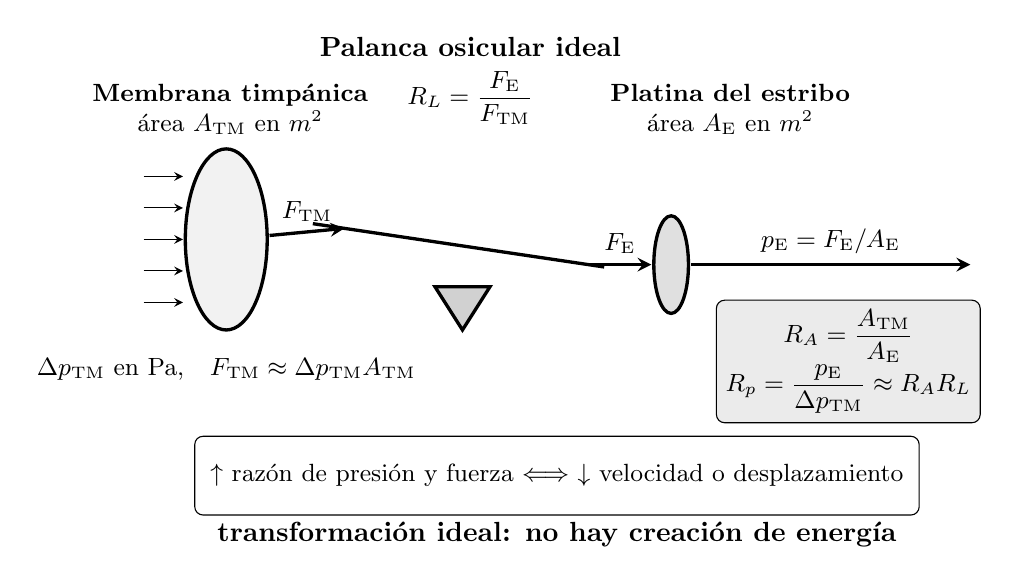
\begin{tikzpicture}[font=\small,>=stealth,x=1cm,y=1cm]
    \tikzset{
        box/.style={draw,rounded corners=3pt,align=center,minimum height=1.0cm},
        flow/.style={->,very thick}
    }

    \draw[very thick,fill=black!5] (1.15,1.90) ellipse (0.52 and 1.15);
    \foreach \yy in {1.10,1.50,1.90,2.30,2.70}{
        \draw[->] (0.10,\yy) -- (0.60,\yy);
    }
    \node[align=center] at (1.20,3.55)
        {\textbf{Membrana timpánica}\\
         área \(A_\mathrm{TM}\) en \(\text{m}^2\)};
    \node[align=center] at (1.15,0.25)
        {\(\Delta p_\mathrm{TM}\) en Pa,\quad
         \(F_\mathrm{TM}\approx\Delta p_\mathrm{TM}A_\mathrm{TM}\)};

    % Palanca ideal.
    \draw[very thick] (2.25,2.10) -- (5.95,1.55);
    \draw[very thick,fill=black!18] (4.15,0.75) -- (3.80,1.30)
        -- (4.50,1.30) -- cycle;
    \draw[flow] (1.70,1.95) -- (2.65,2.04)
        node[midway,above] {\(F_\mathrm{TM}\)};
    \draw[flow] (5.75,1.58) -- (6.55,1.58)
        node[midway,above] {\(F_\mathrm{E}\)};
    \node[font=\bfseries] at (4.25,4.35)
        {Palanca osicular ideal};
    \node at (4.25,3.70)
        {\(\displaystyle R_L=\frac{F_\mathrm{E}}{F_\mathrm{TM}}\)};

    % Platina del estribo.
    \draw[very thick,fill=black!12] (6.80,1.58) ellipse (0.22 and 0.62);
    \node[align=center] at (7.55,3.55)
        {\textbf{Platina del estribo}\\
         área \(A_\mathrm{E}\) en \(\text{m}^2\)};
    \draw[flow] (7.05,1.58) -- (10.60,1.58)
        node[midway,above] {\(p_\mathrm{E}=F_\mathrm{E}/A_\mathrm{E}\)};
    \node[box,fill=black!8,minimum width=3.25cm] at (9.05,0.35)
        {\(\displaystyle R_A=\frac{A_\mathrm{TM}}{A_\mathrm{E}}\)\\
         \(\displaystyle R_p=\frac{p_\mathrm{E}}{\Delta p_\mathrm{TM}}
             \approx R_A R_L\)};

    \node[box,fill=white,minimum width=9.20cm] at (5.35,-1.10)
        {\(\uparrow\) razón de presión y fuerza
         \(\Longleftrightarrow\)
         \(\downarrow\) velocidad o desplazamiento};
    \node[font=\bfseries] at (5.35,-1.85)
        {transformación ideal: no hay creación de energía};
\end{tikzpicture}
